% This file is part of the DDD project.
% Copyright 2014 David W. Hogg (NYU).

\documentclass{beamer}

\setbeamertemplate{footline}[text line]{%
  \parbox{\linewidth}{\vspace*{-8pt}~\hfill David W. Hogg~/~\insertpagenumber}}
\setbeamertemplate{navigation symbols}{}

\newcommand{\foreign}[1]{\textsl{#1}}
\newcommand{\etal}{\foreign{et\,al}}
\renewcommand{\emph}[1]{\textbf{#1}}
\newcommand{\project}[1]{\textsl{#1}}
\newcommand{\Kepler}{\project{Kepler}}

\begin{document}

\begin{frame}
  \frametitle{David W. Hogg}
  \begin{itemize}
  \item go deep-ish on extra-Solar planets
    \begin{itemize}
    \item high-level (planet populations) to low-level (detector pixels)
    \item there are gains available at every level
    \item probailistic inference is my primary technology
    \end{itemize}
  \item other astrophysics projects
  \item methods projects
  \end{itemize}
\end{frame}

\begin{frame}
  \frametitle{David W. Hogg}
  \begin{itemize}
  \item \textsl{Professor of Physics,}\\ New York University
  \item \textsl{Adjunct Senior Staff Scientist,}\\ Max-Planck-Institut f\"ur Astronomie, Heidelberg
  \item \textsl{Executive Director,}\\ Moore--Sloan Data Science Environment at NYU
  \item \textsl{Deputy Director,}\\ NYU Center for Data Science
  \end{itemize}
\end{frame}

\begin{frame}
  \frametitle{Extra-Solar planets: How we find them}
  \begin{itemize}
  \item direct imaging \textit{(ten-ish)}
  \item radial velocity \textit{(hundreds)}
  \item \emph{transit} \textit{(thousands)}
    \begin{itemize}
    \item NASA \Kepler\ Satellite
    \item Earth: \emph{84~ppm} (0.000084) signal for 13~h, once per year
    \end{itemize}
  \item astrometry \textit{(zero, for now, but\ldots)}
  \end{itemize}
\end{frame}

\begin{frame}
  \frametitle{Earth and Jupiter analogs}
  \begin{itemize}
  \item because life!
  \item because Solar-System formation!
  \item in \emph{principle}, \Kepler\ is sensitive enough
    \begin{itemize}
    \item some ``habitable planets'' known
    \item all around stars cooler (and smaller) than the Sun
    \end{itemize}
  \end{itemize}
\end{frame}

\begin{frame}
  \frametitle{Exoplanet populations \small{(Foreman-Mackey \etal)}}
  \begin{itemize}
  \item noisy measurements of a bunch of planets
  \item subject to non-trivial completeness or censoring
  \item how to infer properties of the ``de-noised'' and complete population?
    \begin{itemize}
    \item fully probabilistic inference
    \item fewer assumptions than any other studies
    \item more flexible models
    \item with Dan Foreman-Mackey (NYU)
    \end{itemize}
  \end{itemize}
\end{frame}

\begin{frame}
  \frametitle{Exoplanet populations \small{(Foreman-Mackey \etal)}}
  \includegraphics<1>[width=\textwidth]{pgm.pdf}
  \includegraphics<2>[height=0.85\textheight]{results-results.pdf}
  \includegraphics<3>[width=\textwidth]{results-rate.pdf}
\end{frame}

\begin{frame}
  \frametitle{Exoplanet populations}
  \begin{itemize}
  \item What changed?
    \begin{itemize}
    \item Reduce the expected number of Earth analogs (bad).
    \item Predict that \Kepler\ contains 9-ish detectable examples (good).
    \end{itemize}
  \end{itemize}
\end{frame}

\begin{frame}
  \frametitle{Other astrophysics projects}
  \begin{itemize}
  \item weak gravitational lensing
    \begin{itemize}
    \item \project{The Tractor}
    \end{itemize}
  \item Milky Way formation and dynamics
    \begin{itemize}
    \item \project{Gaia} and \project{APOGEE}
    \end{itemize}
  \item calibration and fundamental astronomy
    \begin{itemize}
    \item \project{Sloan Digital Sky Survey}
    \item \project{Euclid}
    \end{itemize}
  \item citizen science with amateur astronomers
    \begin{itemize}
    \item \project{Astrometry.net}
    \item \project{Open Source Sky Survey}
    \end{itemize}
  \end{itemize}
\end{frame}

\begin{frame}
  \frametitle{NASA \Kepler\ Satellite}
  \includegraphics<1>[width=0.49\textwidth]{750603main_Ball_Kepler_A8468_275_lg_blog_main_horizontal.jpg}%
  \includegraphics<1>[width=0.49\textwidth]{Kepler_FOV_hiRes.jpg}
  \includegraphics<2>[height=0.85\textheight]{FirstLightLogInvertedPink_wslbld2400.jpg}
\end{frame}

\begin{frame}
  \frametitle{NASA \Kepler\ Satellite}
  \begin{itemize}
  \item stared at one patch of sky for 4.1~yr, exposure every 30~min
  \item $10^5$ measurements per star, $10^5$ stars
  \item optimized for stable photometric measurements
    \begin{itemize}
    \item 10~ppm \emph{precision}
    \item but both the s/c and stars vary!
    \end{itemize}
  \end{itemize}
\end{frame}

\begin{frame}
  \frametitle{Flexible models and marginalization \small{(Foreman-Mackey \etal)}}
  \begin{itemize}
  \item stars vary stochastically
    \begin{itemize}
    \item variability driven by turbulent convection
    \item ``filtered'' by response of the star and photosphere
    \end{itemize}
  \item this is a source of structured noise
    \begin{itemize}
    \item correlated (covariant) non-independent noise in the data
    \item non-trivial time history to stellar brightness
    \end{itemize}
  \item Methodology: \emph{Gaussian Processes}
    \begin{itemize}
    \item fastest code in the world for dense kernel-matrix operations (HODLR)
    \item with Dan Foreman-Mackey (NYU), Sivaram Ambikasaran (NYU), Mike O'Neil (NYU)
    \end{itemize}
  \end{itemize}
\end{frame}

\begin{frame}
  \frametitle{flexible models and marginalization \small{(Foreman-Mackey \etal)}}
  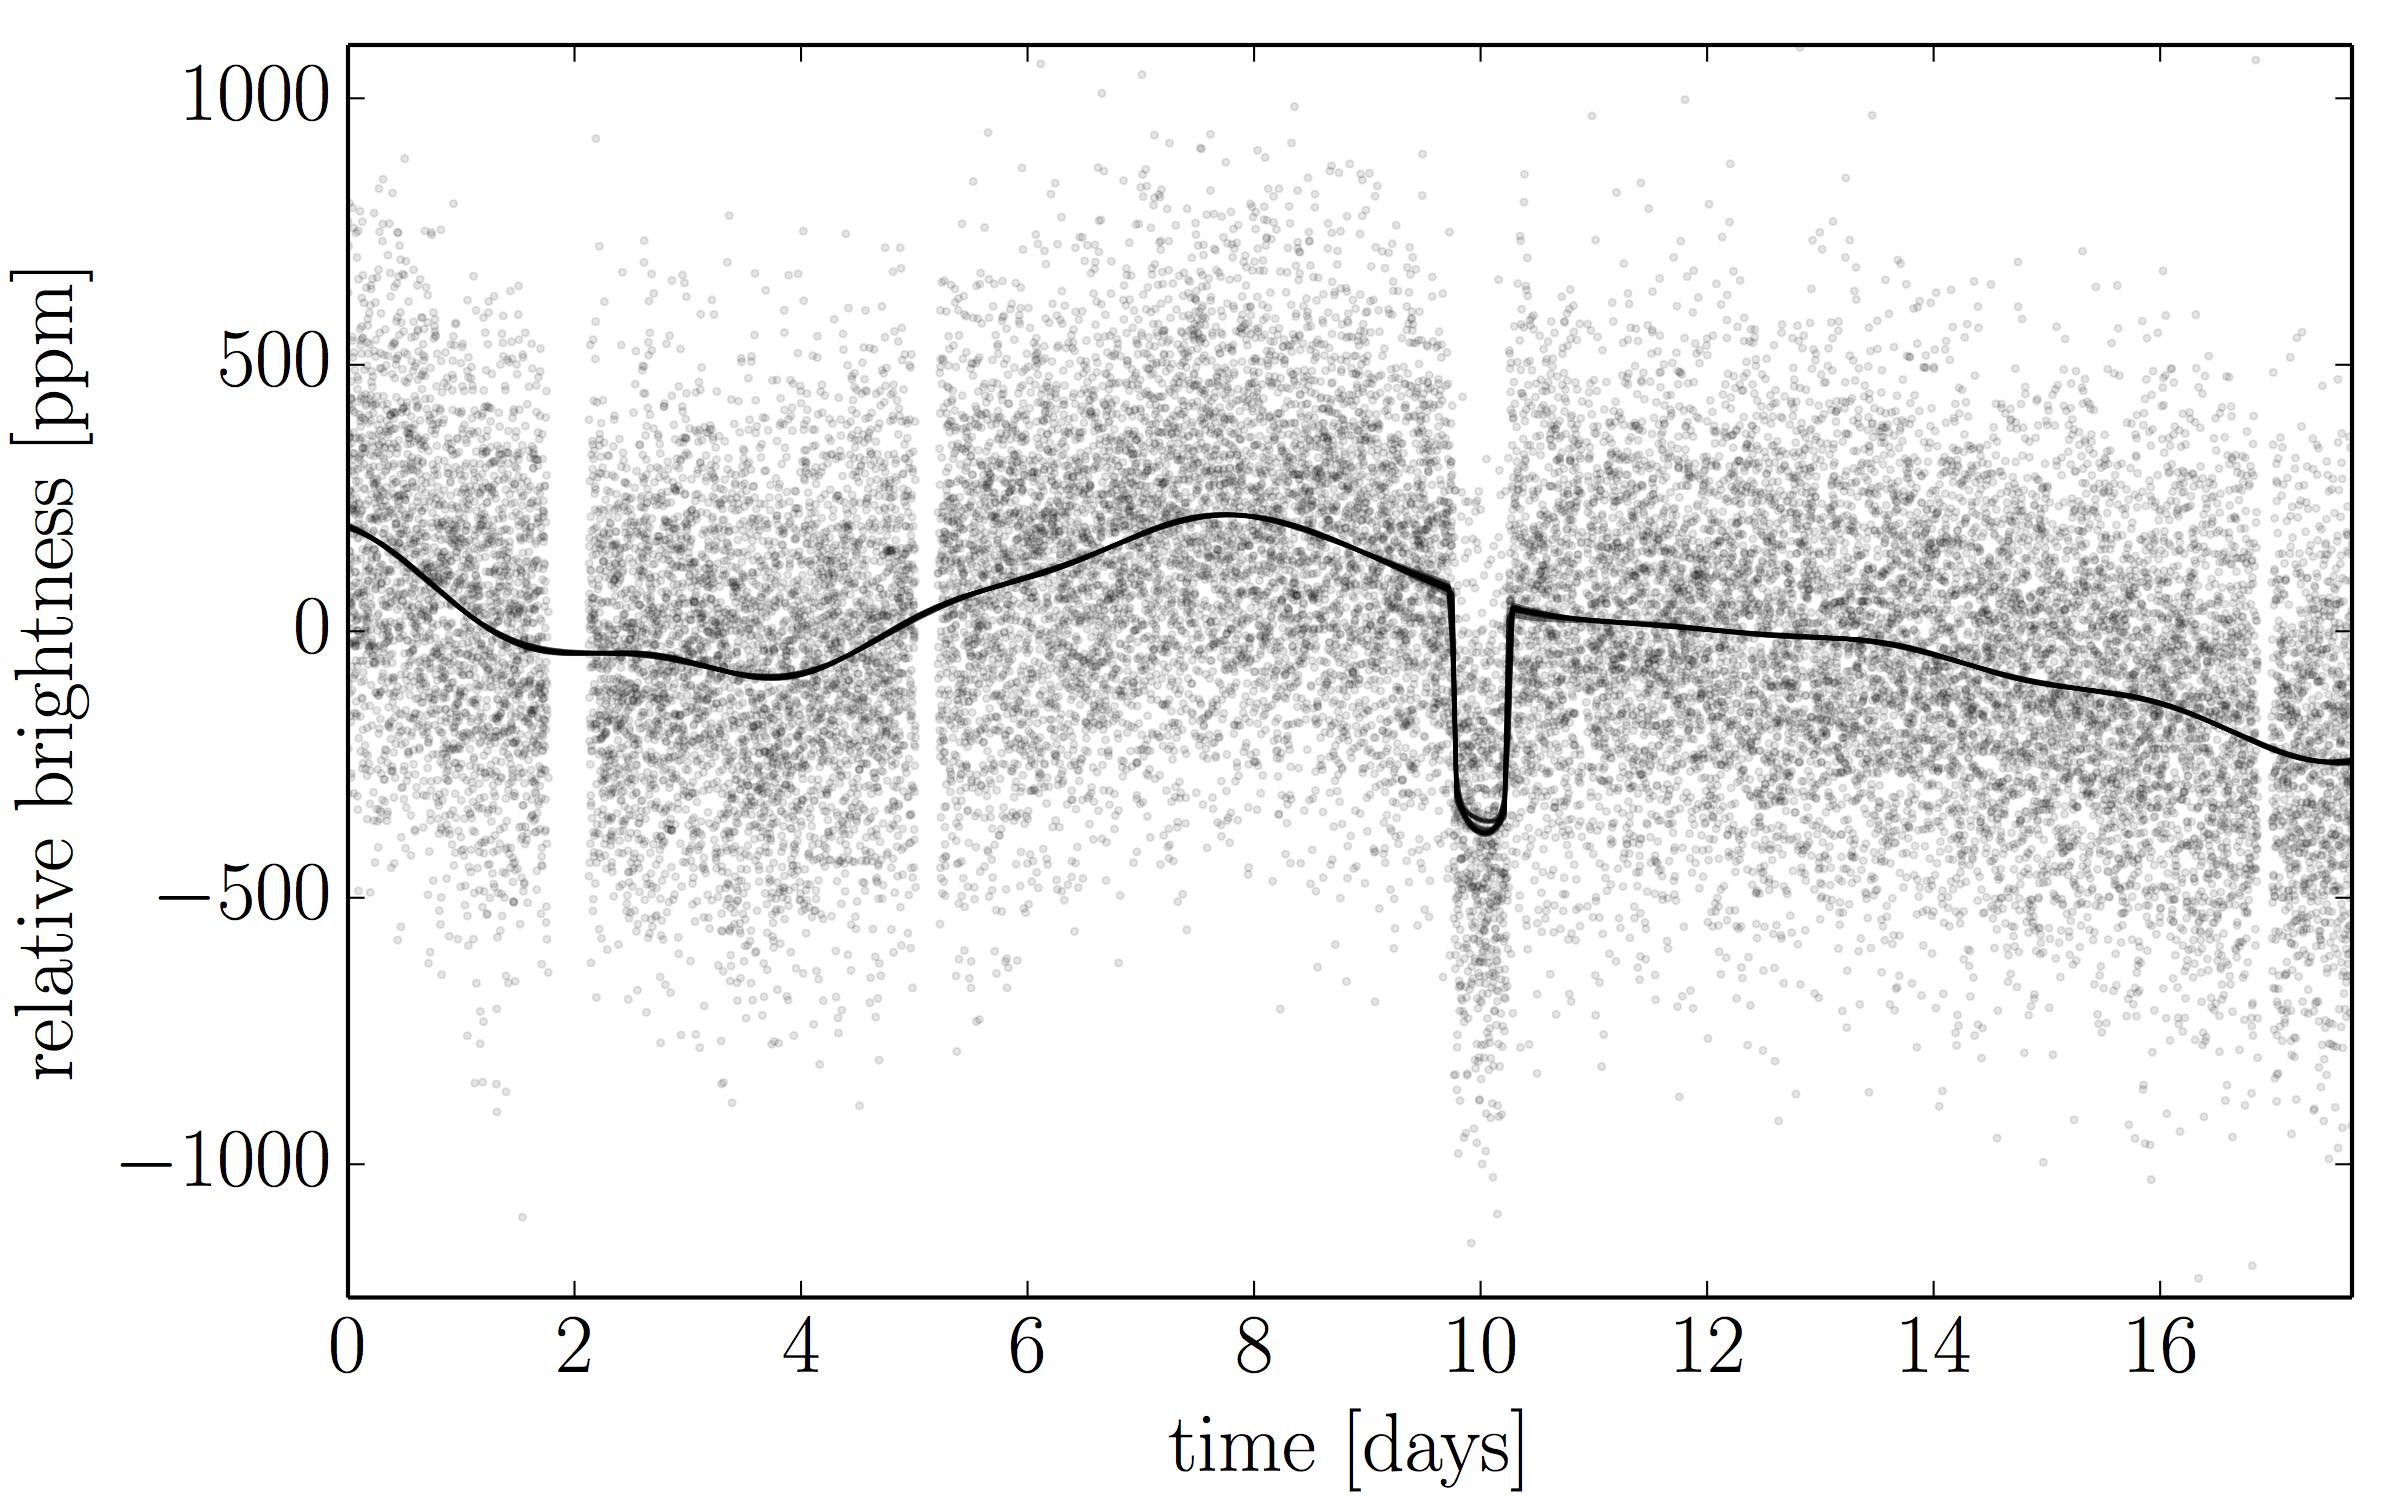
\includegraphics[width=\textwidth]{kepler-prediction.png}
\end{frame}

\begin{frame}
  \frametitle{Flexible models and marginalization \small{(Barclay \etal)}}
  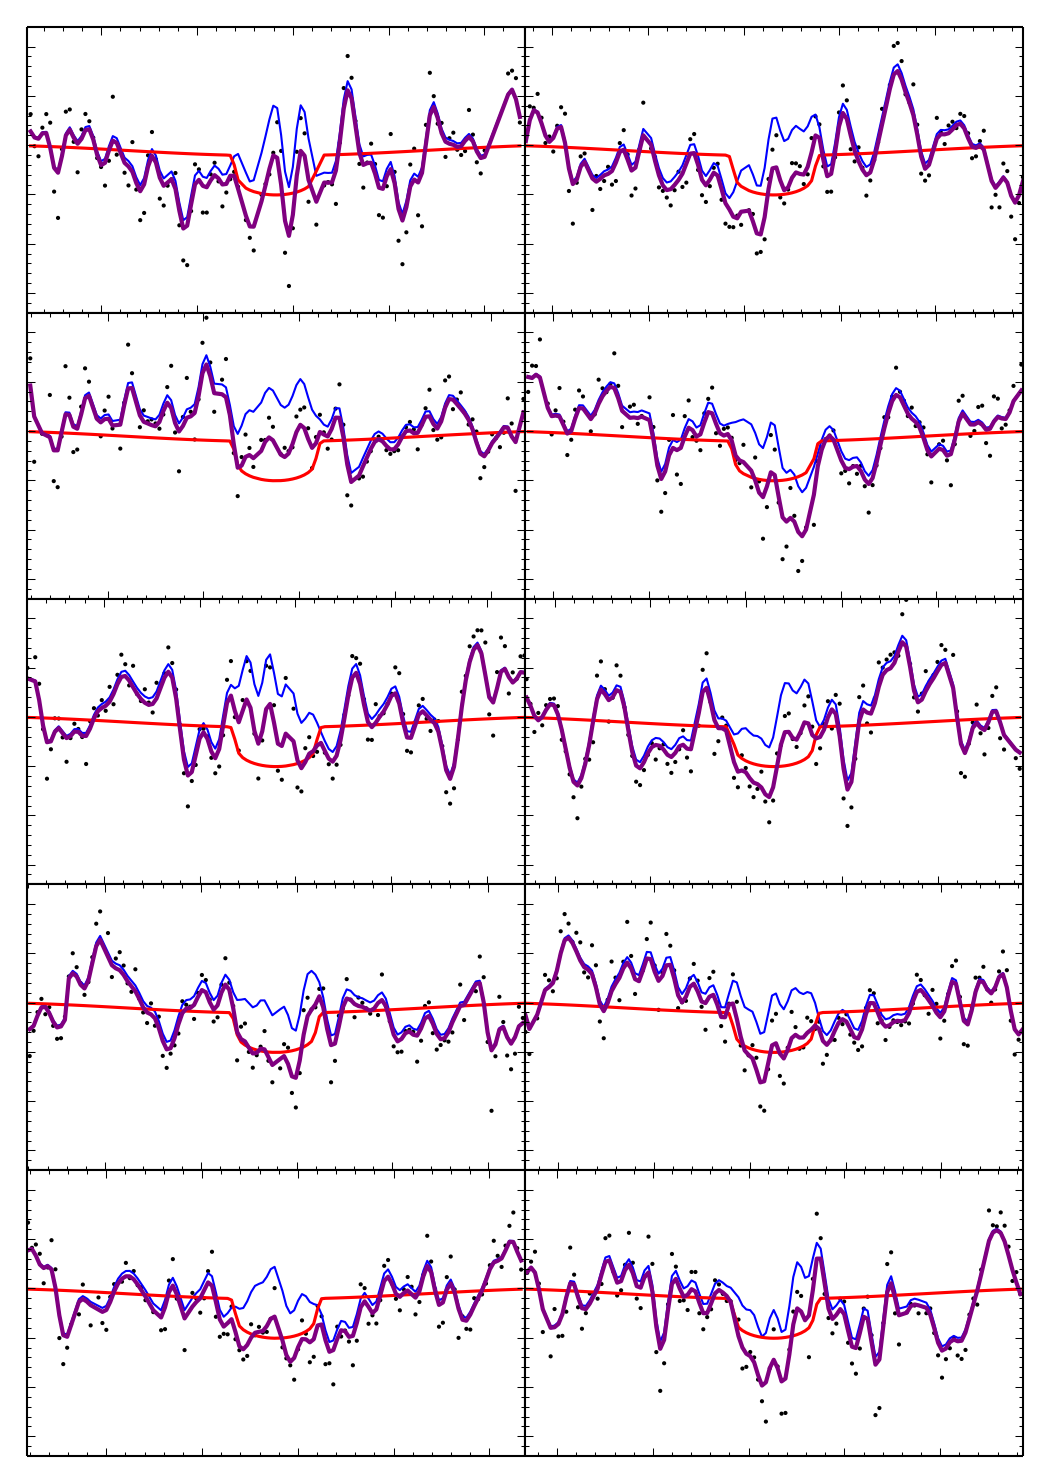
\includegraphics[height=0.85\textheight]{ten_transits.png}
\end{frame}

\begin{frame}
  \frametitle{Flexible models and marginalization}
  \begin{itemize}
  \item What changed?
    \begin{itemize}
    \item Can \emph{marginalize out} the stellar variability.
    \item Can perform inferences on extremely variable stars.
    \end{itemize}
  \end{itemize}
\end{frame}

\begin{frame}
  \frametitle{Methods projects}
  \begin{itemize}
  \item new MCMC methodologies
    \begin{itemize}
    \item with Jonathan Goodman (NYU Mathematics)
    \item \project{emcee} (top-10-cited astrophysics paper from 2013)
    \end{itemize}
  \item computer vision meets astronomy
    \begin{itemize}
    \item with Rob Fergus (NYU Computer Science)
    \item with Bernhard Sch\"olkpf (T\"ubingen MPI-IS)
    \end{itemize}
  \item causal inference and astrophysics
    \begin{itemize}
    \item with Bernhard Sch\"olkpf (T\"ubingen MPI-IS)
    \item with Jennifer Hill (NYU PRIISM)
    \end{itemize}
  \item hierarchical modeling for dummies
    \begin{itemize}
    \item with Brendon Brewer (Auckland Statistics)
    \end{itemize}
  \item fast linear algebra ($n\,\log^2n$) for kernel matrices
    \begin{itemize}
    \item with Sivaram Ambikasaran (NYU Mathematics)
    \item with Mike O'Neil (NYU Mathematics)
    \end{itemize}
  \end{itemize}
\end{frame}

\begin{frame}
  \frametitle{NASA \Kepler\ Satellite}
  \begin{itemize}
  \item stared at one patch of sky for 4.1~yr, exposure every 30~min
  \item only downlinked tiny fraction of $8\times 10^7$ pixels
  \item tens of pixels per star
  \item fixed pointing (by quarter)
    \begin{itemize}
    \item optimal for photometric stability
    \item \emph{pessimal} for self-calibration
    \end{itemize}
  \item \project{K2}, \project{TESS}
  \end{itemize}
\end{frame}

\begin{frame}
  \frametitle{Data-driven self-calibration \small{(Wang \etal)}}
  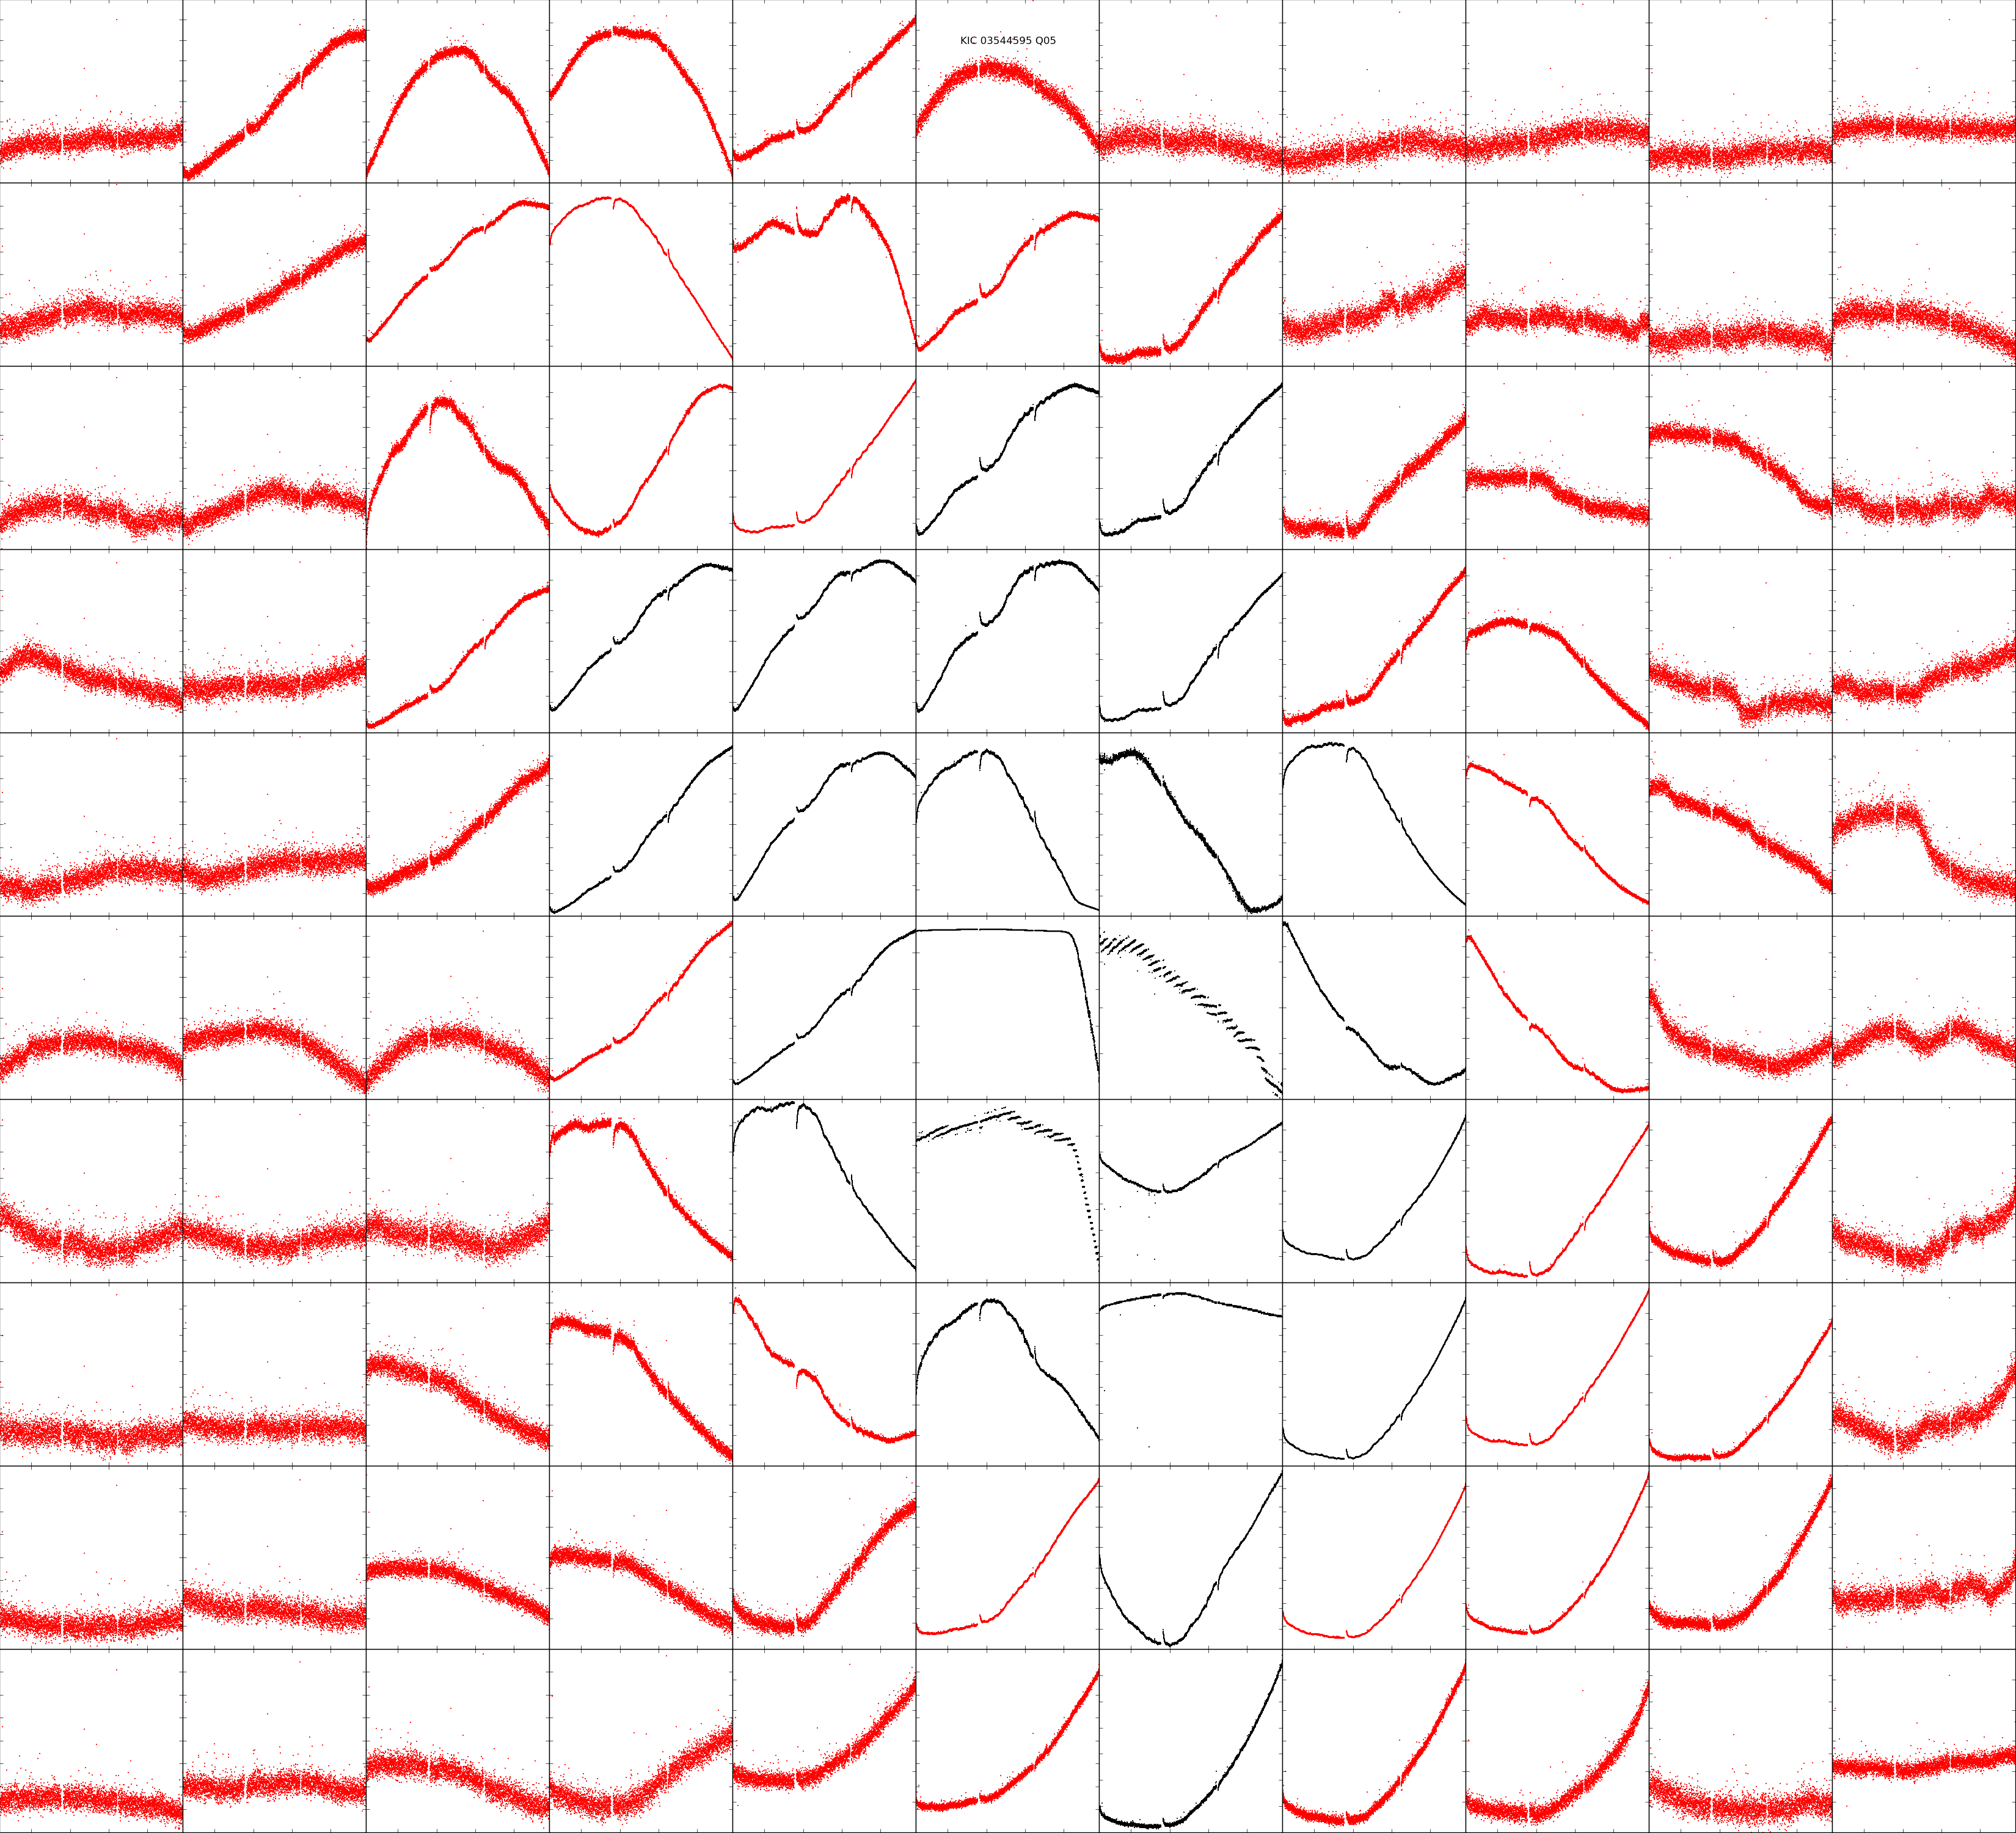
\includegraphics[height=0.85\textheight]{kic_03544595_05_pixels.png}
\end{frame}

\begin{frame}
  \frametitle{Data-driven self-calibration \small{(Wang \etal)}}
  \begin{itemize}
  \item capitalize on \emph{causal structure} of the problem
    \begin{itemize}
    \item variations widely separated pixels have \emph{in common} must be induced by spacecraft variability
    \end{itemize}
  \item massive regression
    \begin{itemize}
    \item using pixels to fit pixels
    \end{itemize}
  \item train-and-test framework
    \begin{itemize}
    \item controlling model complexity
    \item with Dun~Wang (NYU), Dan~Foreman-Mackey (NYU), Bernhard~Sch\"olkopf (T\"ubingen MPI-IS)
    \end{itemize}
  \end{itemize}
\end{frame}

\begin{frame}
  \frametitle{Data-driven self-calibration \small{(Wang \etal)}}
  \includegraphics<1>[width=\textwidth]{lightCurve_5088536_1_90_q5_reg1e+05_pdc_outlier.png}
  \includegraphics<2>[width=\textwidth]{lightCurve_5088536_1_5_q5_reg0e+00_pdc_outlier.png}
\end{frame}

\begin{frame}
  \frametitle{Data-driven self-calibration}
  \begin{itemize}
  \item What will change?
    \begin{itemize}
    \item Improved signal-to-noise on all transits.
    \item Interpretable feedback on s/c hardware.
    \end{itemize}
  \end{itemize}
\end{frame}

\begin{frame}
  \frametitle{Time-domain astronomy}
  \begin{itemize}
  \item top priority for astrophysics in the next decades
    \begin{itemize}
    \item exoplanets, supernovae, asteroseismology, light echos
    \item \project{LSST}, \project{Gaia}, \project{Euclid}, \project{WFIRST}
    \end{itemize}
  \item \textit{not going to talk about it, but ask me!}
  \end{itemize}
\end{frame}

\begin{frame}
  \frametitle{Open Science}
  \begin{itemize}
  \item my group runs \emph{wide open}
    \begin{itemize}
    \item open svn, github, blogging
    \item \url{https://github.com/davidwhogg/DDD}
    \end{itemize}
  \item \textit{not going to talk about it, but ask me!}
  \end{itemize}
\end{frame}

\begin{frame}
  \frametitle{Reclaim of ``engineering''}
  \begin{itemize}
  \item astronomers tend to think of ``engineering'' as ``hardware''
  \item all projects are \emph{integrated hardware--software systems}
    \begin{itemize}
    \item theory, design, build, operations, data handling, inference, legacy
    \item probabilistic modeling is a key technology for all components
    \item my lab is a data analysis shop working on the full ``scientific stack'' (planets to pixels, for example)
    \end{itemize}
  \end{itemize}
\end{frame}

\end{document}
